\chapter{Pași necesari pentru a reproduce}

Informații despre replicarea condițiilor necesare execuției programului scris folosind F* se pot găsi pe pagina de github a limbajului F*. \footnote{https://github.com/FStarLang/FStar/blob/master/INSTALL.md}

În secțiunea următoare se prezintă pașii care au fost luați pentru crearea \newline mediului în care s-a dezvoltat 'SAT solver-ul'. Instrucțiunile următoare sunt \newline compatibile cu sistemul de operare Windows, verificat cu versiunile 10/11. 

\section{Programe si resurse necesare}

Următoarele aplicații/programe/resurse trebuie descărcate de la locația specificată fiecăreia în fișierul 'INSTALL.md' găsit pe pagina de github a limbajului FStar.

\begin{itemize}
 \item OCaml - necesar compilării și executării fișierelor OCaml (.ml), care rezultă în urma compilării fișierelor FStar (.fst)
	(versiune folosita - 4.14.0)
 \item opam - folosit pentru a instala pachetele necesare compilării fișierelor specifice limbajului de programare OCaml 
 
 (versiunea folosită pentru lucrare - 2.0.10)
 \item cygwin - oferă posibilitatea compilării si executării a programelor tipice \newline sistemelor de operare Unix si Linux, ceea ce include suport pentru fișiere \newline  'Makefile' 
 (versiunea folosită pentru lucrare - 3.4.6)
 \item Z3 - folosit pentru a valida fișierele ce conțin programe scrise folosind F*
 
 (arhiva folosită pentru Windows - z3-4.8.5-x64-win.zip)
\end{itemize}

\newpage


După descărcarea/instalarea acestor resurse, trebuie clonată ramura 'master' a proiectului FStar pe dispozitivul local. (locația clonei pe dispozitivul folosit pentru acest proiect: "D:/fstar", versiunea  - F* 2023.04.26~dev )

Trebuie adăugate path-urile absolute către ".../fstar/bin" si ".../z3-win/bin" in variabila 'Path' a sistemului.

După instalarea programului 'opam', trebuie instalate anumite pachete de date. Minimul necesar de pachete se poate găsi si pe instrucțiunile de instalare găsite la link-ul de mai sus, însă pentru a avea la dispoziție toate resursele din proiectul FStar descarcat fără erori, sunt necesare următoarele pachete: 
\newline

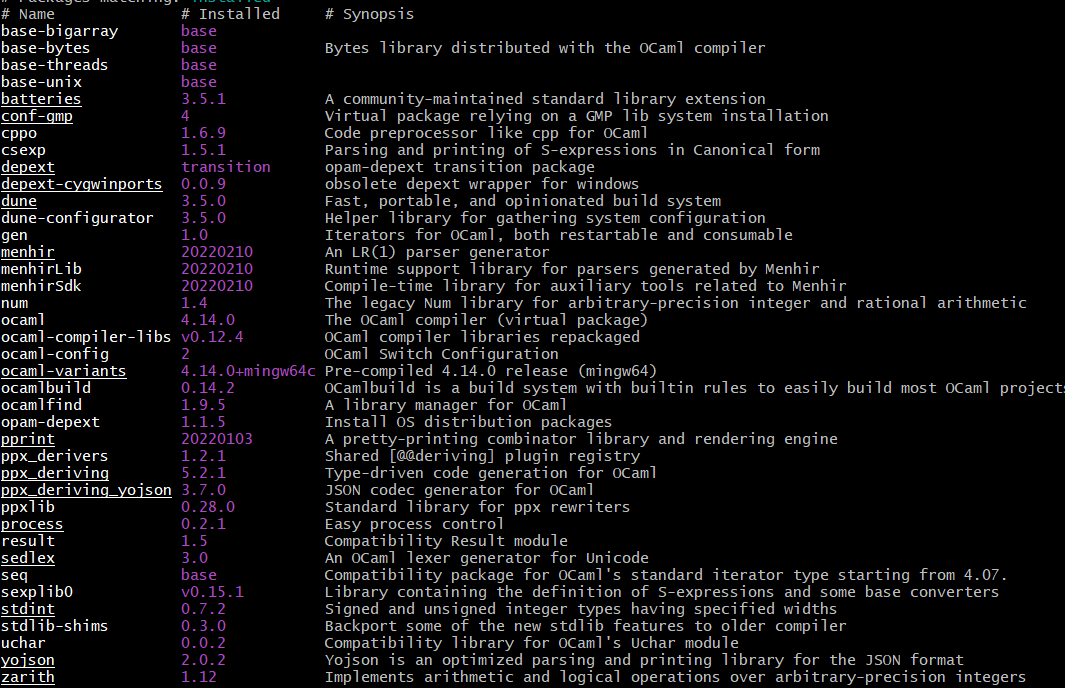
\includegraphics[width=1\textwidth]{opam_necesary_packages.png}
\newline

La finalul acestor pași, folosind terminalul Cygwin și instrucțiunile de tipul 'make' în folder-ul 'fstar', ar trebui să funcționeze verificarea și executarea oricăror fișiere surse scrise în F*, fișiere proprii sau exemple ce făceau deja parte din proiect.

\newpage

\section{Executarea solver-ului SAT}

Sursele corespunzătoare proiectului prezentat se găsesc la:
\href{https://github.com/alex4482/FStar-DPLL-licenta/tree/main/dpll_optimized}{FStar-DPLL github}.

Aceste surse trebuie descărcate, salvate într-un folder în proiectul 'fstar'. \newline Fișierul 'Makefile' trebuie modificat, astfel încât variabila 'FSTAR-HOME'  să facă \newline referire spre folder-ul 'fstar'. Același pas trebuie făcut pentru fișieru 'Makefile' din \newline folder-ul 'output'.

Apoi, în terminalul cygwin deschis în folder-ul proiectului DPLL-FStar, trebuie executată comanda 'make', la finalul căreia în folder-ul 'output' vor apărea pentru \newline fiecare fișier sursă '.fst', câte un fișier '.ml', iar acestea conțin codul Ocaml extras din sursele FStar. De asemenea în folder-ul 'output' se va afla executabilul "Main.exe".

Pentru a recompila si regenera fișierul "Main.exe", trebuie șters cel anterior creat, dacă a fost creat.

Imediat după pornirea programului "Main.exe", trebuie introdus de la tastatură calea relativă către un fișier de input. Câteva fișiere de input există în folder-ul \newline "input-files" și orice alt fișier de intrare trebuie să respecte acea structură pentru ca parsarea implementată a datelor să funcționeze.

La finalul unei astfel de execuții, va apărea mesaj la consolă cu rezultatul obținut, fie că formula dată este nesatisfiabilă, fie că e satisfiabilă si alături o variantă de răspuns ce conține variabilele formulei si valorile lor booleene astfel încât fiecare clauză a formulei să aibe valoarea de adevăr \textit{true}.
\newline

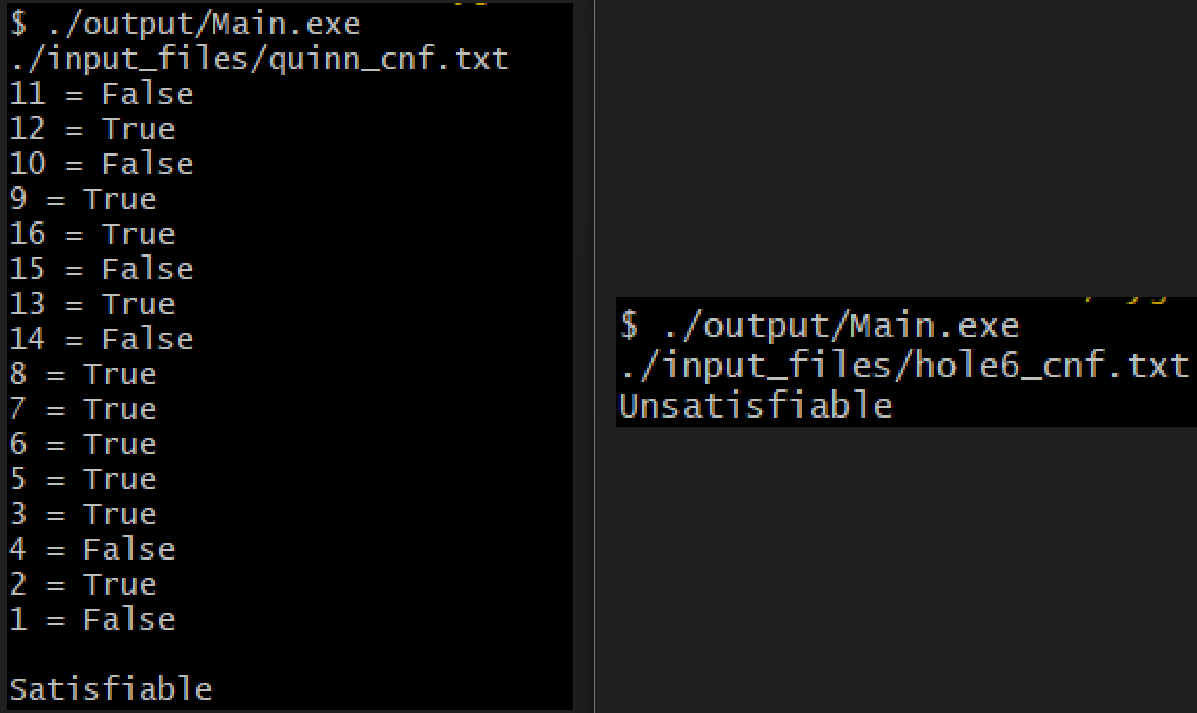
\includegraphics[width=0.8\textwidth]{unsat-sat-result-execute-example.png}

